\documentclass[dutch]{beamer}
\usepackage{babel}
\usepackage{graphicx}
\usepackage{epsfig}
\usepackage{color}
\usepackage{algorithmic}
\usepackage{multicol}

\usetheme{Rochester}
\useinnertheme{rounded}
\usefonttheme{structurebold}
\usecolortheme{beetle}

\newtheorem{stelling}[theorem]{Stelling}

\theoremstyle{definition}
\newtheorem{definitie}[theorem]{Definitie}

\theoremstyle{remark}
\newtheorem{opmerking}[theorem]{Opmerking}

\theoremstyle{example}
\newtheorem{voorbeeld}[theorem]{Voorbeeld}


\AtBeginSection[]{\plainframe{\tableofcontents[currentsection,hidesubsections]}}

\title{Similariteitsgebaseerd rangschikken van beelden in zoekmachines}
\author{Klaas Bosteels}
\date{Academiejaar 2005-2006}

\titlegraphic{\includegraphics[scale=1]{ugent.eps}}

\begin{document}

\plainframe{\titlepage}

\section{Inleiding}
\subsection{Situering}
\frame
{
  \frametitle{Situering}
  
  \begin{center}
  \includegraphics[width=\textwidth]{images/situering.eps}
  \end{center}
}
\subsection{Tekstgebaseerd zoeken van beelden}
\frame
{
  \frametitle{Tekstgebaseerd zoeken van beelden}

  \begin{center}
  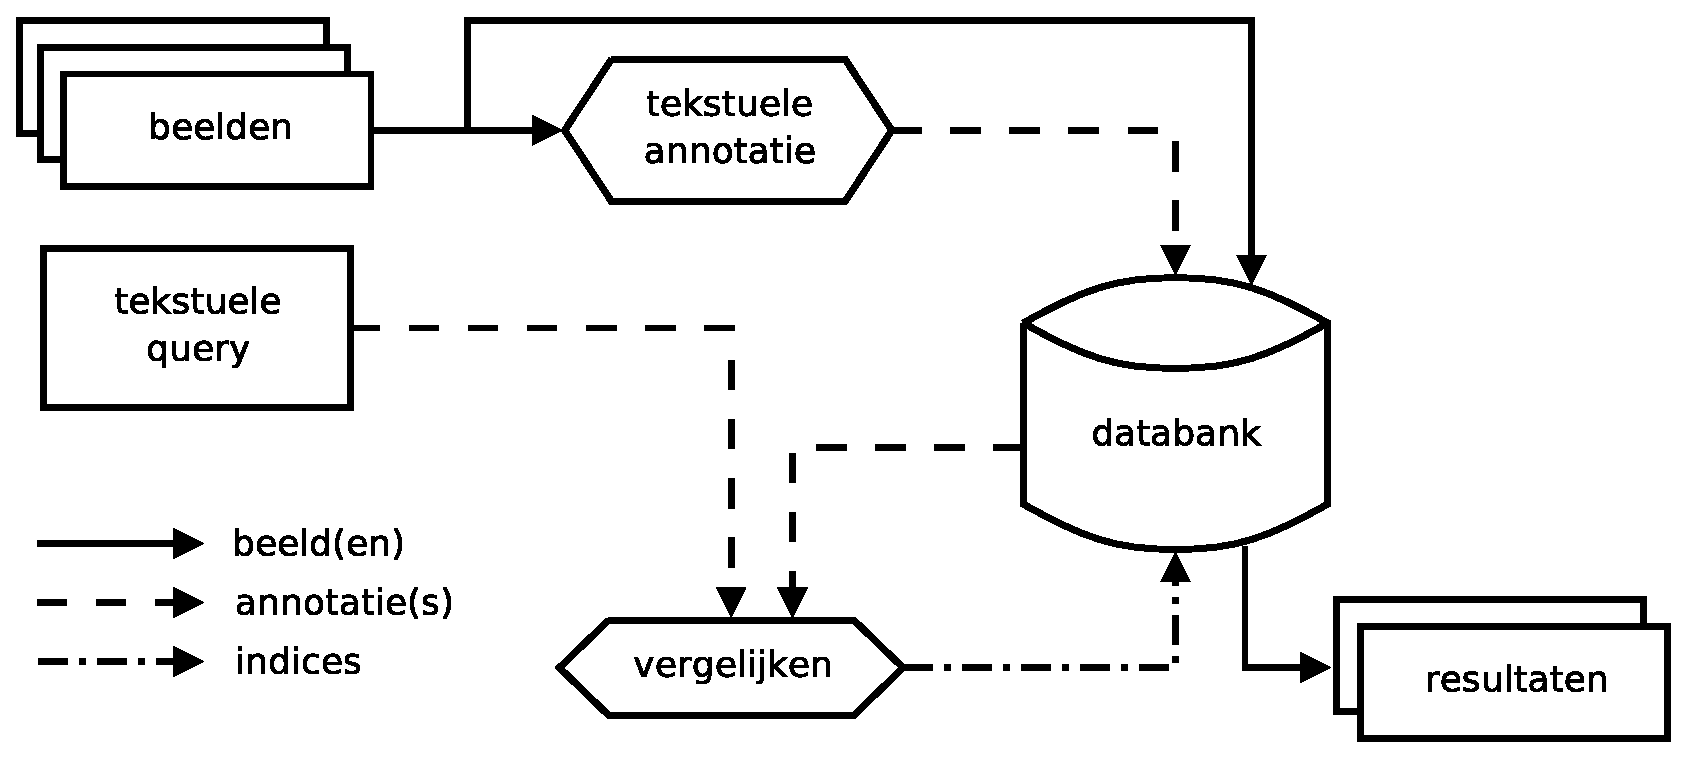
\includegraphics[width=\textwidth]{images/tbir.eps}
  \end{center}

  Terminologie: Text-Based Image Retrieval (TBIR).
}
\subsection{Inhoudgebaseerd zoeken van beelden}
\frame
{
  \frametitle{Inhoudgebaseerd zoeken van beelden}

  \begin{center}
  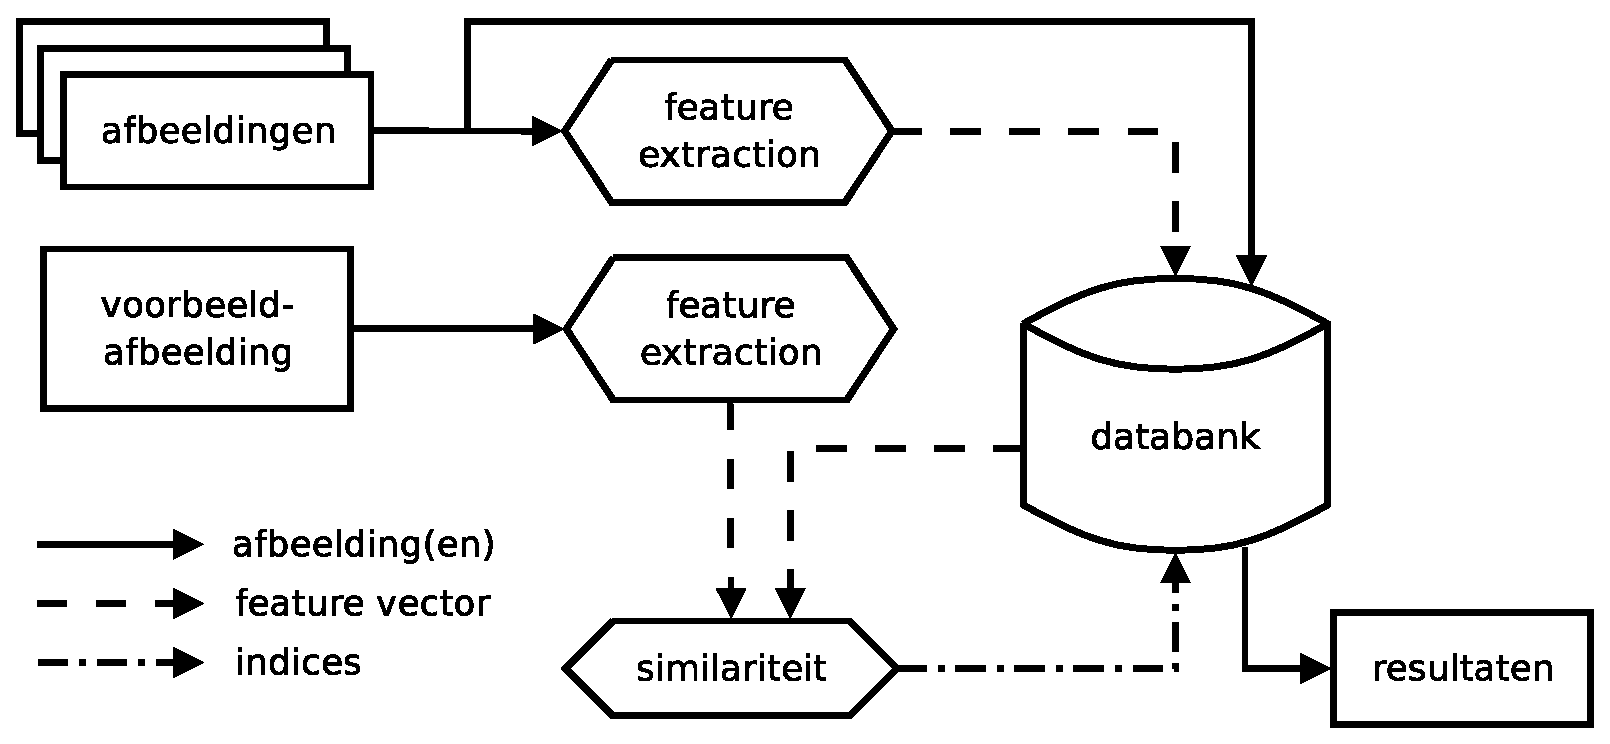
\includegraphics[width=\textwidth]{images/cbir.eps}
  \end{center}

  Terminologie: Content-Based Image Retrieval (CBIR).
}
\subsection{Similariteitsgebaseerd rangschikken van de zoekresultaten}
\frame
{
  \frametitle{Similariteitsgebaseerd rangschikken van de zoekresultaten}
  
  \begin{itemize}
  \item Nadelen CBIR:
  \begin{enumerate}
    \item Te complex voor zeer omvangrijke databanken.
    \item Gebruiker beschikt niet altijd over een geschikt voorbeeld.
  \end{enumerate}

  \item Alternatief:
  \begin{center}
  \includegraphics[width=0.8\textwidth]{images/simgeb_rangschikken.eps}
  \end{center}
  Extra laag bovenop TBIR die ervoor zorgt dat de resultaten gerangschikt
  worden volgens similariteit met een opgegeven verzameling van voorbeelden.
  \end{itemize}
}

% \section{Enkele begrippen uit beeldverwerking}
% \subsection{Modellering van kleuren en beelden}
% \frame
% {
%   \frametitle{Modellering van kleuren en beelden}
%   
%   \centering
%   \begin{tabular}{@{}lr@{}}
%   \begin{minipage}{0.7\textwidth}
%   \begin{itemize}
%     \item \textbf{Kleurmodel}: abstract mathematisch model dat beschrijft
%     hoe kleuren gerepresenteerd kunnen worden als $n$-tallen uit $\mathbb{R}^n$.
%     \begin{itemize}
%     \item Voorbeelden: RGB, HSV en L*a*b*.
%     \end{itemize}
%     \item De kleuren die op basis van een bepaald model kunnen voorgesteld worden, vormen
%     een \textbf{kleurruimte}.
%     \begin{itemize}
%       \item Voorbeelden: sRGB, Adobe RGB.
%     \end{itemize}
%     \item Als we de $n$-tallen uit het
%     kleurmodel normaliseren tot $n$-tallen uit $[0,1]^n$, dan kunnen we een
%     tweedimensionaal kleurbeeld modelleren als een $\mathbb{N}^2 - [0,1]^n$
%     afbeelding.
%   \end{itemize}
%   \end{minipage} &
%   \begin{minipage}{0.3\textwidth}
%   \centering
%   \includegraphics[height=2.2cm]{images/rgb.eps}\\
%   \includegraphics[height=2.2cm]{images/hsv.eps}\\[2pt]
%   \includegraphics[height=2.2cm]{images/lab.eps}
%   \end{minipage}
%   \end{tabular}
% }
% \subsection{Kleurkwantisatie}
% \frame
% {
%   \frametitle{Kleurkwantisatie}
%   \begin{itemize}
%     \item \textbf{Kleurkwantisatie}: het aantal kleuren in een kleurruimte 
%     reduceren.
%     \item Principe:
%     \begin{enumerate}
%       \item De kleuren groeperen in zogenaamde \textbf{bins}.
%       \item Alle kleuren van een bin vervangen door \'e\'en enkele kleur.
%     \end{enumerate}
%     \item Wiskundig:
%     \begin{enumerate}
%     \item $C - \{1,2,\ldots,N\}$ afbeelding $bin$: associeert met elke kleur uit de 
%     kleurruimte $C$ het nummer van de corresponderende bin.
%     \item $\{1,2,\ldots,N\} - C$ afbeelding $col$: bepaalt de kleur van elke bin.
%     \end{enumerate}
%     \item \textbf{Uniforme kwantisatie}: 
%     \begin{itemize}
%       \item Elke kleurcomponent wordt uniform verdeeld in een aantal intervallen. 
%       \item De middelste waarden van de intervallen doen dienst
%       als componenten van de kleur van een bin.
%     \end{itemize}
%   \end{itemize}
% }
% \definecolor{zwart}{rgb}{0,0,0}
% \definecolor{blauw}{rgb}{0,0,1}
% \definecolor{groen}{rgb}{0,1,0}
% \definecolor{rood}{rgb}{1,0,0}
% \definecolor{bruin}{rgb}{0.5,0.16,0.16}
% \definecolor{oranje}{rgb}{1,0.5,0}
% \definecolor{geel}{rgb}{1,1,0}
% \definecolor{paars}{rgb}{0.62,0.125,0.94}
% \definecolor{grijs}{rgb}{0.75,0.75,0.75}
% \definecolor{roze}{rgb}{1,0.75,0.79}
% \definecolor{wit}{rgb}{1,1,1}
% \frame
% {
%   \frametitle{Beschouwde kwantisatietechnieken}
%   
%   \begin{itemize}
%   \item Zes manieren om uniform te kwantiseren, waarbij we telkens een ander
%   kleurmodel gebruiken.
%   \item Vier niet-uniforme kwantisatietechnieken:
%   \begin{enumerate}
%     \item \textbf{Smooth Color Transition (SCT) kwantisatie}: combinatie van twee uniforme
%     kwantisaties, \'e\'en voor grijstinten en \'e\'en voor kleurtinten. Als 
%     $s > 1 - 0.8\cdot v$ dan wordt de kleur benaderd met een kleurtint en anders met een
%     grijstint.
%     \item Afbeelding naar elf \textbf{focale kleuren} ({\color{zwart}zwart}, 
%     {\color{blauw}blauw}, {\color{groen}groen}, {\color{rood}rood}, 
%     {\color{bruin}bruin}, {\color{oranje}oranje}, {\color{geel}geel}, 
%     {\color{paars}paars}, {\color{grijs}grijs}, {\color{roze}roze} en {\color{wit}wit}): 
%     elke kleur vervangen door de focale kleur die het meest
%     nabij licht in het perceptueel uniforme L*a*b*-model.
%     \item \textbf{Neural Image Quantization (NeuQuant)}, waarbij gebruik gemaakt wordt van een 
%     Kohonen neuraal netwerk.
%     \item \textbf{Wu kwantisatie}, die gebaseerd is op dynamisch programmeren en principal 
%     component analysis.
%   \end{enumerate}
%   \end{itemize}
% }
% \frame
% {
%   \frametitle{Voorbeelden}
% 
%   \begin{center}
%   \begin{tabular}{@{}c@{\ }c@{\ }c@{\ }c@{\ }c@{\ }c@{}}
%   \includegraphics[width=0.15\textwidth]{images/uniform_hsv_flowers.eps} &
%   \includegraphics[width=0.15\textwidth]{images/uniform_irb_flowers.eps} &
%   \includegraphics[width=0.15\textwidth]{images/uniform_i1i2i3_flowers.eps} &
%   \includegraphics[width=0.15\textwidth]{images/uniform_xyz_flowers.eps} &
%   \includegraphics[width=0.15\textwidth]{images/uniform_yxy_flowers.eps} &
%   \includegraphics[width=0.15\textwidth]{images/uniform_lab_flowers.eps} \\
%   HSV & Irb & I1I2I3 & XYZ & Yxy & L*a*b* \\
%   {\scriptsize $16 \cdot 4 \cdot 4$} & {\scriptsize $4 \cdot 8 \cdot 8$} & 
%   {\scriptsize $4 \cdot 8 \cdot 8$} & {\scriptsize $8 \cdot 4 \cdot 8$} &
%   {\scriptsize $4 \cdot 8 \cdot 8$} & {\scriptsize $4 \cdot 8 \cdot 8$} \vspace{5pt}\\
%   \includegraphics[width=0.15\textwidth]{images/sct_flowers.eps} &
%   \includegraphics[width=0.15\textwidth]{images/focal_flowers.eps} &
%   \includegraphics[width=0.15\textwidth]{images/neuquant_flowers.eps} &
%   \includegraphics[width=0.15\textwidth]{images/wu_flowers.eps} &
%   \includegraphics[width=0.15\textwidth]{images/neuquant_flowers_8.eps} &
%   \includegraphics[width=0.15\textwidth]{images/wu_flowers_8.eps} \\
%   SCT & focaal & NeuQuant & Wu & NeuQuant & Wu \\
%   {\scriptsize $256$} & {\scriptsize $11$} & 
%   {\scriptsize $256$} & {\scriptsize $256$} &
%   {\scriptsize $8$} & {\scriptsize $8$}
%   \end{tabular}
%   \end{center}
% 
%   \begin{center}
%   \begin{tabular}{@{}rl@{}}
%   \begin{minipage}{0.5\textwidth}
%   \centering
%   \includegraphics[width=\textwidth]{images/probleem_focale_kwantisatie.eps}\\
%   \end{minipage} &
%   \begin{minipage}{0.3\textwidth}
%   \raggedright
%   Onverwachte omzetting bij focale kwantisatie.
%   \end{minipage}
%   \end{tabular}
%   \end{center}
% }

\section{Similariteitsmaten voor beelden}
\subsection{Definitie en eigenschappen}
\frame
{
  \frametitle{Definitie en eigenschappen}

  \begin{itemize}
  \item \textbf{Similariteitsmaat voor beelden:} maat die de gelijkenis 
  tussen twee gegeven beelden uitdrukt als een getal uit het eenheidsinterval 
  $[0,1]$.
  \item We construeren similariteitsmaten voor beelden door:
  \begin{enumerate}
    \item beelden te identificeren met (L-)vaagverzamelingen en
    \item gebruik te maken van vaagsimilariteitsmaten om die (L-)vaagverzamelingen
    te vergelijken.
  \end{enumerate}
  \item Eigenschappen:
  \begin{itemize}
  \item Reflexief: $M(A,A)=1$
  \item Symmetrisch: $M(A,B)=M(B,A)$
  \item Geen (vorm van) transitiviteit, want dat zou bijvoorbeeld impliceren dat 
  het eerste en het laatste beeld van
  \begin{center}
  \vspace{5pt}
  \includegraphics[width=0.8cm]{images/video_trans_1.eps}\ 
  \includegraphics[width=0.8cm]{images/video_trans_2.eps}\ 
  \includegraphics[width=0.8cm]{images/video_trans_3.eps}\ 
  \includegraphics[width=0.8cm]{images/video_trans_4.eps}\ 
  \includegraphics[width=0.8cm]{images/video_trans_5.eps}\
  \includegraphics[width=0.8cm]{images/video_trans_6.eps}\
  \ldots\ 
  \includegraphics[width=0.8cm]{images/video_trans_10.eps}\ 
  \includegraphics[width=0.8cm]{images/video_trans_11.eps}
  \end{center}
  zeer similair zijn, wat niet overeenkomt met onze intu\"itie.
  \end{itemize}
  \end{itemize}
}
\subsection{Evaluatie van performantie}
\frame
{
  \frametitle{Evaluatie van performantie}

  Testcollectie van $N$ beelden die corresponderen met 
  $N/N_R$ objecten die elk $N_R$ keer gefotografeerd werden:

\begin{center}

\begin{tabular}{c@{\ }c@{}c@{}c@{}c@{}c c@{\ }c@{}c@{}c@{}c@{}c}

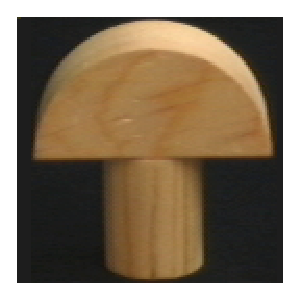
\includegraphics[width=0.8cm]{coil/beeld-0.eps} &
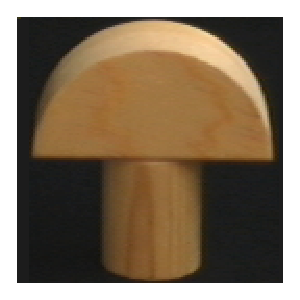
\includegraphics[width=0.8cm]{coil/beeld-1.eps} &
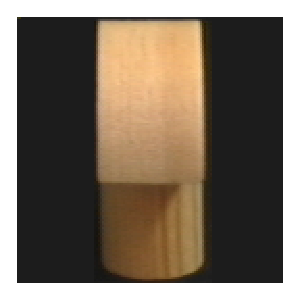
\includegraphics[width=0.8cm]{coil/beeld-2.eps} &
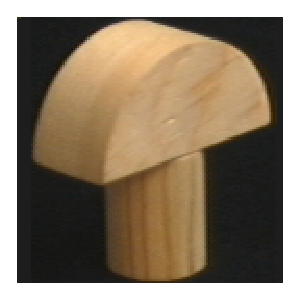
\includegraphics[width=0.8cm]{coil/beeld-3.eps} &
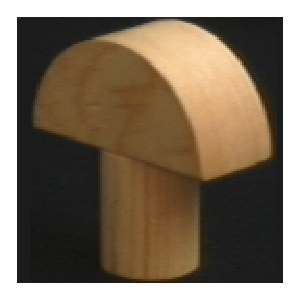
\includegraphics[width=0.8cm]{coil/beeld-4.eps} &
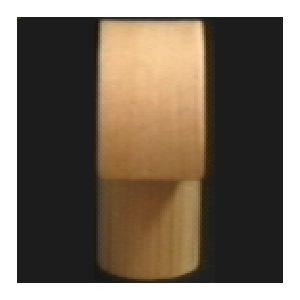
\includegraphics[width=0.8cm]{coil/beeld-5.eps} &

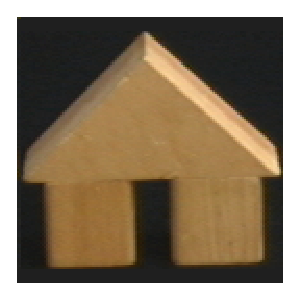
\includegraphics[width=0.8cm]{coil/beeld-42.eps} &
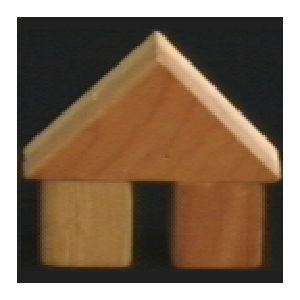
\includegraphics[width=0.8cm]{coil/beeld-43.eps} &
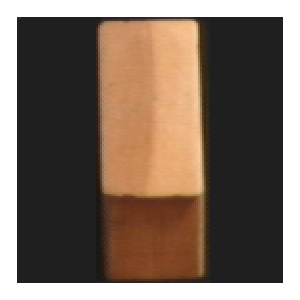
\includegraphics[width=0.8cm]{coil/beeld-44.eps} &
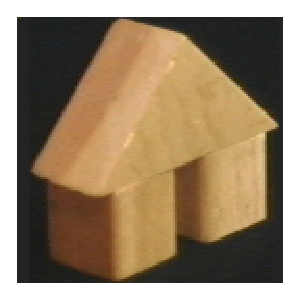
\includegraphics[width=0.8cm]{coil/beeld-45.eps} &
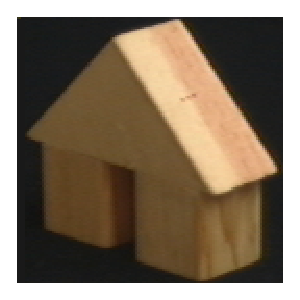
\includegraphics[width=0.8cm]{coil/beeld-46.eps} &
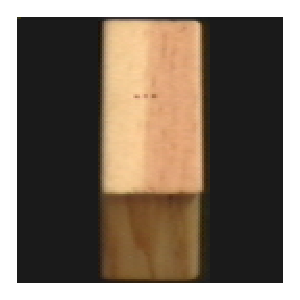
\includegraphics[width=0.8cm]{coil/beeld-47.eps} \\

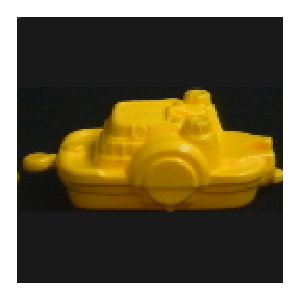
\includegraphics[width=0.8cm]{coil/beeld-12.eps} &
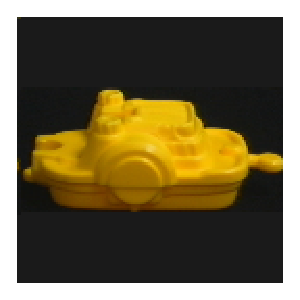
\includegraphics[width=0.8cm]{coil/beeld-13.eps} &
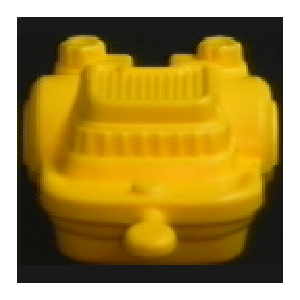
\includegraphics[width=0.8cm]{coil/beeld-14.eps} &
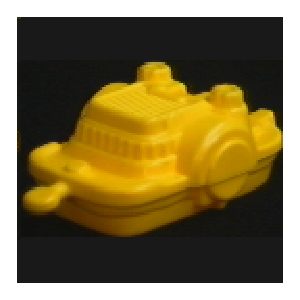
\includegraphics[width=0.8cm]{coil/beeld-15.eps} &
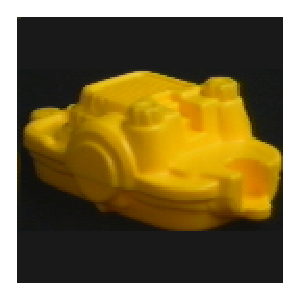
\includegraphics[width=0.8cm]{coil/beeld-16.eps} &
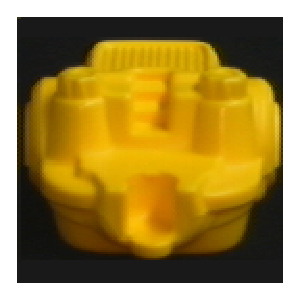
\includegraphics[width=0.8cm]{coil/beeld-17.eps} &


\includegraphics[width=0.8cm]{coil/beeld-18.eps} &

\includegraphics[width=0.8cm]{coil/beeld-19.eps} &
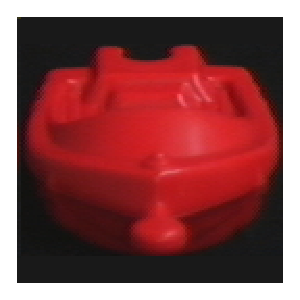
\includegraphics[width=0.8cm]{coil/beeld-20.eps} &
\includegraphics[width=0.8cm]{coil/beeld-21.eps} &
\includegraphics[width=0.8cm]{coil/beeld-22.eps} &
\includegraphics[width=0.8cm]{coil/beeld-23.eps} \\

\includegraphics[width=0.8cm]{coil/beeld-24.eps} &
\includegraphics[width=0.8cm]{coil/beeld-25.eps} &
\includegraphics[width=0.8cm]{coil/beeld-26.eps} &
\includegraphics[width=0.8cm]{coil/beeld-27.eps} &
\includegraphics[width=0.8cm]{coil/beeld-28.eps} &
\includegraphics[width=0.8cm]{coil/beeld-29.eps} &

\includegraphics[width=0.8cm]{coil/beeld-54.eps} &
\includegraphics[width=0.8cm]{coil/beeld-55.eps} &
\includegraphics[width=0.8cm]{coil/beeld-56.eps} &
\includegraphics[width=0.8cm]{coil/beeld-57.eps} &
\includegraphics[width=0.8cm]{coil/beeld-58.eps} &
\includegraphics[width=0.8cm]{coil/beeld-59.eps} \\

\includegraphics[width=0.8cm]{coil/beeld-30.eps} &
\includegraphics[width=0.8cm]{coil/beeld-31.eps} &
\includegraphics[width=0.8cm]{coil/beeld-32.eps} &
\includegraphics[width=0.8cm]{coil/beeld-33.eps} &
\includegraphics[width=0.8cm]{coil/beeld-34.eps} &
\includegraphics[width=0.8cm]{coil/beeld-35.eps} &

\includegraphics[width=0.8cm]{coil/beeld-36.eps} &
\includegraphics[width=0.8cm]{coil/beeld-37.eps} &
\includegraphics[width=0.8cm]{coil/beeld-38.eps} &
\includegraphics[width=0.8cm]{coil/beeld-39.eps} &
\includegraphics[width=0.8cm]{coil/beeld-40.eps} &
\includegraphics[width=0.8cm]{coil/beeld-41.eps} \\

\includegraphics[width=0.8cm]{coil/beeld-6.eps} &
\includegraphics[width=0.8cm]{coil/beeld-7.eps} &
\includegraphics[width=0.8cm]{coil/beeld-8.eps} &
\includegraphics[width=0.8cm]{coil/beeld-9.eps} &
\includegraphics[width=0.8cm]{coil/beeld-10.eps} &
\includegraphics[width=0.8cm]{coil/beeld-11.eps} &

\includegraphics[width=0.8cm]{coil/beeld-48.eps} &
\includegraphics[width=0.8cm]{coil/beeld-49.eps} &
\includegraphics[width=0.8cm]{coil/beeld-50.eps} &
\includegraphics[width=0.8cm]{coil/beeld-51.eps} &
\includegraphics[width=0.8cm]{coil/beeld-52.eps} &
\includegraphics[width=0.8cm]{coil/beeld-53.eps} \\

\includegraphics[width=0.8cm]{coil/beeld-60.eps} &
\includegraphics[width=0.8cm]{coil/beeld-61.eps} &
\includegraphics[width=0.8cm]{coil/beeld-62.eps} &
\includegraphics[width=0.8cm]{coil/beeld-63.eps} &
\includegraphics[width=0.8cm]{coil/beeld-64.eps} &
\includegraphics[width=0.8cm]{coil/beeld-65.eps} &
\multicolumn{2}{c}{$N_R = 6$} & 
\multicolumn{4}{c}{$N = 11 \cdot N_R = 66$}

\end{tabular}
\end{center}

}
\frame
{
  \frametitle{Evaluatie van performantie}

  \begin{itemize}
  \item De \textbf{genormaliseerde gemiddelde rang} (GGR) wordt gegeven door de volgende afbeelding:
  \begin{minipage}{\textwidth}
  \vspace{3pt}
  \centering
  \scriptsize$\begin{array}{lrcl}
  \text{GGR}: & \{1,2,\ldots,N\}^{N_R} & \to 	& [0,1] \\
		& (r_1,r_2,\ldots,r_{N_R}) & \mapsto &
	{\displaystyle\frac{1}{N \cdot N_R}\left[ \left(\sum_{i=1}^{N_R}r_i\right) - \frac{N_R \cdot (N_R + 1)}{2} \right]},\\[15pt]
	& & & \qquad \quad \forall (r_1, r_2, ..., r_{N_R}) \in \{1,2,\ldots,N\}^{N_R}
  \end{array}$
  \end{minipage}
  \item Evaluatie:
  \begin{enumerate}
    \item De te evalueren similariteitsmaat gebruiken om de testcollectie te rangschikken 
    volgens similariteit met een voorbeeld. 
    \item $\text{GGR}(r_1,r_2,\ldots,r_{N_R})$ berekenen, waarbij $r_i$ het rangnummer 
    van het $i$-de relevante beeld voorstelt. Hoe groter de bekomen waarde, hoe 
    slechter de performantie.
  \end{enumerate}
  \item Voorbeeld voor onze testcollectie:
  \begin{itemize}
    \item Stel dat alle relevante beelden vooraan gerangschikt worden: 
    $(r_1,r_2,\ldots,r_6) = (1,2,\ldots,6)$.
    \item Dan: $\text{GGR}(1,2,\ldots,6)=\frac{1}{66 \cdot 6} \left[21 - \frac{6 \cdot 7}{2}\right]=0$
  \end{itemize}
  \end{itemize}
}
\frame
{
  \frametitle{Evaluatie van performantie}

  \begin{itemize}
  \item De GGR kan een verkeerd beeld geven omdat de performantie afhankelijk
  kan zijn van het gekozen voorbeeld. 
  \item \textbf{Globale genormaliseerde gemiddelde rang} (GGGR): gemiddelde van
  de GGRs voor
  \begin{center}
  \vspace{5pt}
  \includegraphics[width=0.8cm]{coil/beeld-0.eps}, 
  \includegraphics[width=0.8cm]{coil/beeld-42.eps}, 
  \includegraphics[width=0.8cm]{coil/beeld-12.eps}, 
  \includegraphics[width=0.8cm]{coil/beeld-18.eps}, 
  \includegraphics[width=0.8cm]{coil/beeld-24.eps}, 
  \includegraphics[width=0.8cm]{coil/beeld-54.eps},\\
  \vspace{5pt}
  \includegraphics[width=0.8cm]{coil/beeld-30.eps}, 
  \includegraphics[width=0.8cm]{coil/beeld-36.eps}, 
  \includegraphics[width=0.8cm]{coil/beeld-6.eps}, 
  \includegraphics[width=0.8cm]{coil/beeld-48.eps}\ en  
  \includegraphics[width=0.8cm]{coil/beeld-60.eps}. 
  \end{center}
  \item Rekentijd: we meten ook hoe lang het duurt om de rangschikkingen, 
  die nodig zijn om de GGGR te bepalen, te berekenen.
  \end{itemize}
}
\subsection{Beperken van de rekentijd}
\frame
{
  \frametitle{Beperken van de rekentijd}
  
  \begin{itemize}
  \item Stel: $A$ en $B$ twee vaagverzamelingen in $X$. 
  \item Als $X'= supp\ A \cup supp\ B$ en $|X'| \ll |X|$, dan kunnen we 
  de rekentijd sterk reduceren door het bereik van de sommaties in de 
  vaagsimilariteitsmaten te beperken tot $X'$. 
  \item Wanneer we $||C|| = \sum_{x \in X'} C(x)$
  defini\"eren voor elke $C \in \mathcal{F}(X)$, dan vinden we bijvoorbeeld:
  \begin{minipage}{\textwidth}
  \vspace{4pt}
  \centering
  \scriptsize
  \begin{tabular}{@{}ccc@{}}
  $M_{7}(A,B) = \displaystyle \frac{|A \cap B|}{\max \{|A|,|B|\}}$ & $\displaystyle\to$ &
  $M_{7}(A,B) = \displaystyle \frac{||A \cap B||}{\max \{||A||,||B||\}}$ \vspace{5pt}\\
  \begin{tabular}{r}
  $|X|+1$ vergelijkingen\\
  $3\cdot (|X|-1)$ optellingen\\
  $1$ deling\\
  \hline
  $4\cdot |X| - 1$
  \end{tabular} & &
  \begin{tabular}{r}
  $|X'|+1$ vergelijkingen\\ 
  $3\cdot (|X'|-1)$ optellingen\\
  $1$ deling\\
  \hline
  $4\cdot |X'| - 1$
  \end{tabular} 
  \end{tabular}
  \vspace{4pt}
  \end{minipage}
  \item Bij de maten die gebruik maken van het complement boeken we nog meer winst
  omdat we bijvoorbeeld $|A^c|$ herschrijven als $|X|-||A||$.
  \end{itemize}
}

\section{Pixelgebaseerde similariteitsmaten}
\subsection{Grijswaardebeelden}
\frame
{
  \frametitle{Pixelgebaseerde similariteitsmaten voor grijswaardebeelden}
%   \begin{definitie}
%   Een tweedimentionaal \textbf{binair beeld} is een eindig rooster dat enkel 
%   witte en zwarte beeldpunten bevat.
%   \end{definitie}
%   Representatie: scherpe verzameling $A$ in $\mathbb{N}^2$ met:
%   \begin{displaymath}
%   \begin{array}{rcl}
%   p \in A & \iff & p \text{ is een wit punt in het beeld} \\
%   p \notin A & \iff & p \text{ is een zwart punt in het beeld}
%   \end{array}
%   \end{displaymath}
%   \begin{definitie}
%   Een tweedimensionaal \textbf{grijswaardebeeld} is een eindig rooster dat
%   naast wit en zwart ook grijstinten kan bevatten.
%   \end{definitie}
  \begin{itemize}
  \item Grijswaardebeeld representeren als een vaagverzameling 
  $A$ in $\mathbb{N}^2$ bepaald door:
  \begin{displaymath}
  \begin{array}{rcl}
  A(p) = 1 & \iff & p \text{ is een wit punt in het beeld} \\
  A(p) = 0 & \iff & p \text{ is een zwart punt in het beeld} \\
  A(p) \in\ ]0,1[ & \iff & p \text{ is een beeldpunt met een grijstint}
  \end{array}
  \end{displaymath}
  waarbij geldt: hoe groter de lidmaatschapsgraad, hoe lichter de grijstint.
  \item Door die representatie te combineren met een vaagsimilariteitsmaat,
  bekomen we een similariteitsmaat voor grijswaardebeelden. 
  \item Omdat het universum daarbij bestaat uit beeldpunten (pixels), spreken we van
  \textbf{pixelgebaseerde} similariteitsmaten.
  \end{itemize}
}
\subsection{Kleurbeelden}
\frame
{
  \frametitle{Pixelgebaseerde similariteitsmaten voor kleurbeelden}
  
  \begin{itemize}
     \item Probleem: de meeste beelden op internet zijn 
     geen grijswaardebeelden maar kleurbeelden.
     \item We beschouwen drie mogelijke oplossingen:
     \begin{enumerate}
       \item Beelden eerst omzetten naar grijswaardebeelden, bijvoorbeeld aan de 
       hand van de formule $0.3 \cdot r + 0.59 \cdot g + 0.11 \cdot b$.
       \item Componentsgewijze aanpak:
       \begin{enumerate}
       \item Een similariteitsmaat voor grijswaardebeelden toepassen op elke
       kleurcomponent. 
       \item De resultaten voor de verschillende componenten
       aggregeren tot \'e\'en getal.
       \end{enumerate}
       \item Traliegebaseerde aanpak:
        \begin{enumerate}
          \item L-vaagverzamelingen gebruiken om kleurbeelden te representeren.
          \item De vaagsimilariteitsmaten uitbreiden zodanig dat ze kunnen
          toegepast worden op die L-vaagverzamelingen.
        \end{enumerate}
     \end{enumerate}
   \end{itemize}
}
% \frame
% {
%   \frametitle{Traliegebaseerde aanpak}
% 
%   \begin{enumerate}
%   \item Kleurbeelden representeren als een L-vaagverzameling in $\mathbb{N}^2$,
%   waarbij we de complete tralie $([0,1]^3, \le_{RGB,lex})$ gebruiken:
%   \begin{minipage}{\textwidth}
%   \vspace{7pt}
%   \scriptsize
%   \centering
%   $\begin{array}{@{}r@{}l@{}}
%    c <_{RGB} c' & \ \iff d(c,Bl) < d(c',Bl)\ \lor \\
% 			 & \ \qquad \qquad (d(c,Bl) = d(c',Bl) \land d(c,Wh) > d(c',Wh)) \\[4pt]
%    c >_{RGB} c' & \ \iff d(c,Wh) < d(c',Wh)\ \lor \\
% 			 & \ \qquad \qquad (d(c,Wh) = d(c',Wh) \land d(c,Bl) > d(c',Bl)) \\[4pt]
%    c =_{RGB} c' & \ \iff (d(c,Bl) = d(c',Bl) \land d(c,Wh) = d(c',Wh)) \\[4pt]
%    c \leq_{lex} c' & \ \iff r < r' \lor (r = r' \land g < g') \lor (r = r' \land g = g' \land b \leq b') \\[4pt]
%    c \leq_{RGB,lex} c' & \ \iff c <_{RGB} c' \lor (c =_{RGB} c' \land c \leq_{lex} c')
%   \end{array}$
%   \vspace{7pt}
%   \end{minipage}
%   met $Bl = (0,0,0)$, $Wh = (1,1,1)$ en $d$ de Euclidische afstand.
%   \item Veralgemenen van de bewerkingen waarvan de vaagsimilariteitsmaten gebruik maken.
%   \begin{itemize}
%     \item Voorbeeld: $|A|=\frac{1}{\sqrt{3}}\sum_{p \in P}\sqrt{(A_1(p))^2+(A_2(p))^2+(A_3(p))^2}$
%     met $A(p)=(A_1(p),A_2(p),A_3(p))$ voor alle $p$ uit het universum der beeldpunten $P$.
%   \end{itemize}
%   \end{enumerate}
% }
\subsection{Resolutie-onafhankelijke similariteitsmaten}
\frame
{
  \frametitle{Resolutie-onafhankelijke similariteitsmaten}
  
  \centering
  \begin{tabular}{@{}cc@{}}
  \begin{minipage}{0.7\textwidth}
  \begin{itemize}
  \item Het aantal pixels in een beeld wordt de \textbf{resolutie} van dat beeld genoemd.
  \item Probleem: de similariteitsmaten die we tot nu toe beschouwd hebben, kunnen 
  enkel toegepast worden op beelden die dezelfde resolutie hebben.
  \item Oplossing: constructie van resolutie-onafhankelijke 
  pixelgebaseerde similariteitsmaten door
  \begin{itemize}
      \item \textbf{intermediaire beelden} of 
      \item \textbf{beeldonderdelen} 
  \end{itemize}
  te beschouwen.
  \end{itemize}
  \end{minipage} &
  \begin{minipage}{0.25\textwidth}
  \includegraphics[width=0.8\textwidth]{images/resolutieprobleem.eps}
  \end{minipage}
  \end{tabular}
}
\frame
{
  \frametitle{Resolutie-onafhankelijke similariteitsmaten: intermediaire beelden}

  \begin{center}
  \begin{tabular}{@{}lc@{}}
  \begin{minipage}{0.6\textwidth}
  De beelden \textbf{herschalen} zodanig dat we twee beelden met dezelfde resolutie bekomen. 
  \end{minipage} & 
  \begin{minipage}{0.4\textwidth}
  \includegraphics[height=0.25\textheight]{images/rescale.eps}
  \end{minipage}\vspace{5pt}\\
  \begin{minipage}{0.6\textwidth}
  Eerst \textbf{kleurkwantisatie} met een variabel kleurenpalet toepassen en vervolgens een
  nieuw beeld construeren op basis van de kleuren van het bekomen palet.
  \end{minipage} &
  \begin{minipage}{0.4\textwidth}
  \includegraphics[height=0.25\textheight]{images/dominant_colors.eps}
  \end{minipage}\vspace{5pt}\\
  \begin{minipage}{0.6\textwidth}
  \textbf{Kleurmomenten} (gemiddelde, variantie en scheefheid) gebruiken om nieuwe 
  intermediaire beelden te construeren.
  \end{minipage} &
  \begin{minipage}{0.4\textwidth}
  \includegraphics[height=0.25\textheight]{images/moments.eps}
  \end{minipage}
  \end{tabular}
  \end{center}
}
\frame
{
  \frametitle{Resolutie-onafhankelijke similariteitsmaten: beeldonderdelen}
  
  \begin{minipage}{\textwidth}
  \centering
  \includegraphics[width=0.65\textwidth]{images/multires.eps}\qquad
  \includegraphics[width=0.25\textwidth]{images/multires_sim-matrix_beide.eps}
  \vspace{4pt}
  \end{minipage}
  Ruwe schets van werking:
  \begin{enumerate}
    \item Beelden partitioneren in beeldonderdelen met dezelfde resolutie 
    ($8 \cdot 8$ pixels).
    \item De beeldonderdelen (van groot naar klein) ordenen op basis van
    hun gemiddelde kleur.
    \item Gebruik maken van de ordening om grote similariteiten te vinden.
    \item Het gemiddelde van de grote similariteiten bepalen.
  \end{enumerate}
}
\subsection{Experimentele observaties}
\frame
{
  \frametitle{Experimentele observaties}
  
  %De GGGR-waarde en de rekentijd in ms voor elk van de similariteitsmaten op basis 
  %van herschaalde beelden:
  \begin{center}
  \begin{tabular}{@{}c@{}c@{}}
  \includegraphics[width=0.5\textwidth]{plots/scaling_gggrs_en_cputimes_filled.eps} &
  \includegraphics[width=0.5\textwidth]{plots/moments_gggrs_en_cputimes_filled.eps}\\
  {\scriptsize intermediaire beelden: herschaling} & {\scriptsize intermediaire beelden: kleurmomenten} \vspace{10pt}\\
  \includegraphics[width=0.5\textwidth]{plots/dom_colors_neuquant_gggrs_en_cputimes_filled.eps} &
  \includegraphics[width=0.5\textwidth]{plots/dom_colors_wu_gggrs_en_cputimes_filled.eps}\\
  {\scriptsize intermediaire beelden: NeuQuant} & {\scriptsize intermediaire beelden: Wu}
  \end{tabular}
  \end{center}
}
\frame
{
  \frametitle{Experimentele observaties}
  
  \begin{center}
  \begin{tabular}{@{}cc@{}}
  \begin{minipage}{0.5\textwidth}
  \begin{tabular}{@{}c@{}}
  \includegraphics[width=\textwidth]{plots/multires_gggrs_en_cputimes_filled.eps}\\
  {\scriptsize beeldonderdelen}
  \end{tabular}
  \end{minipage} &
  \begin{minipage}{0.4\textwidth}
  \raggedright
  De gegevens in de onderstaande tabel werden berekend uit de GGGRs van alle 
  pixelgebaseerde similariteitsmaten die we beschouwd hebben.
  \end{minipage} \vspace{10pt}
  \end{tabular}
  \end{center}

  \begin{center}
  \tiny
  \begin{tabular}{r|cccccccc}
  & $M_{1a}$ & $M_{1b}$ & $M_{1c}$ & $M_{2}$ & $M_{3}$ & $M_{5}$ & $M_{5c}$ & $M_{6}$ \\
  \hline
  minimale GGGR & 0.0147 & 0.0245 & 0.0323 & 0.0355 & 0.0093 & 0.0128 & 0.0219 & 0.0102 \\
  gemiddelde GGGR & 0.0818 & 0.0951 & 0.1115 & 0.1428 & {\color{white} 0.0802} & 0.0922 & 0.0971 & 0.1024\vspace{8pt}\\
  & $M_{6c}$ & $M_{7}$ & $M_{7c}$ & $M_{8}$ & $M_{8c}$ & $M_{9}$ & $M_{9c}$ & $M_{10}$ \\
  \hline
  minimale GGGR & 0.0212 & 0.0089 & 0.0203 & 0.2024 & 0.1985 & {\color{white} 0.0084} & 0.0201 & 0.2212 \\
  gemiddelde GGGR & 0.1145 & 0.0873 & 0.0922 & 0.3604 & 0.3688 & 0.0806 & 0.0868 & 0.3895\vspace{8pt}\\
  & $M_{10c}$ & $M_{11}$ & $M_{11c}$ & $M_{12}$ & $M_{13}$ & $M_{I_3}$ & $M_{I_{3c}}$ \\
  \hline
  minimale GGGR & 0.2106 & 0.0128 & 0.0219 & 0.0203 & 0.1985 & 0.0102 & 0.0212 \\
  gemiddelde GGGR & 0.3850 & 0.0922 & 0.0971 & 0.0922 & 0.3696 & 0.1035 & 0.1038
  \end{tabular}
  \end{center} 
}
\frame
{
  \frametitle{Experimentele observaties}
  
%   Tot nu toe hebben we telkens het gemiddelde gebruikt om te aggregeren bij
%   de componentsgewijze aanpak. We kunnen echter ook een t-norm gebruiken.
%   De beelden kunnen dan enkel similair 
%   zijn indien \emph{alle} kleurcomponenten goed op elkaar lijken.
  
  \begin{center}
  \begin{tabular}{@{}c@{}c@{}}
  \includegraphics[width=0.5\textwidth]{plots/dom_colors_wu_comps_gggrs_en_cputimes_filled.eps} &
  \includegraphics[width=0.5\textwidth]{plots/moments_comps_gggrs_en_cputimes_filled.eps}\\
  {\scriptsize intermediaire beelden: Wu} & {\scriptsize intermediaire beelden: kleurmomenten}
  \end{tabular}
  \end{center}

  \begin{itemize}
  \item Aggregeren met een t-norm (in plaats van het gemiddelde) bij de componentsgewijze 
  aanpak: beelden kunnen enkel similair zijn indien \emph{alle} kleurcomponenten 
  goed op elkaar lijken.
  \item Intermediaire beelden
  op basis van kleurmomenten componentsgewijs vergelijken met behulp van 
  \begin{enumerate}
    \item het minimum en 
    \item $M_3$, $M_6$, $M_7$ of $M_{I_3}$ 
  \end{enumerate} geeft de beste resultaten.
  \end{itemize}
}
\frame
{
  \frametitle{Verklaringen voor observaties}
  
  \begin{itemize}
  \item \textbf{Valse positieven}: verkeerdelijk hoge similariteiten tussen
  sterk verschillende beelden. 
  \item \textbf{Valse negatieven}: lage similariteiten tussen zeer gelijkaardige
  beelden.
  \item Het optreden van valse positieven is de oorzaak van de volgende observaties:
  \begin{enumerate}
    \item De componentsgewijze aanpak werkt beter dan de traliegebaseerde
    methode.
    \item De vaagsimilariteitsmaten $M_8$, $M_{8c}$, $M_{10}$, $M_{10c}$ en $M_{13}$ 
    geven systematisch aanleiding tot de minst performante maten.
    \item Bij de componentsgewijze aanpak kunnen we betere resultaten bekomen als we 
    aggregeren met een t-norm in plaats van het gemiddelde.
  \end{enumerate}
  \end{itemize}
}

\section{Kleurgebaseerde similariteitsmaten}
\subsection{Histogrammen}
\frame
{
  \frametitle{Kleurgebaseerde similariteitsmaten}

  \begin{itemize}
  \item Bij \textbf{kleurgebaseerde} similariteitsmaten bestaat het universum
  uit kleuren in plaats van beeldpunten. 
  \item Om de complexiteit te beperken,
%   beperken we daarbij het aantal kleuren met behulp van kleurkwantisatie.
%   De gekwantiseerde versie van het universum der kleuren $C$ noemen we $C'$. 
  reduceren we het universum der kleuren $C$ tot $C'$ met behulp van
  \textbf{kleurkwantisatie}:
  \begin{itemize}
  \item Principe:
  \begin{enumerate}
   \item De kleuren groeperen in zogenaamde \textbf{bins}.
   \item Alle kleuren van een bin vervangen door \'e\'en enkele kleur.
  \end{enumerate}
  \item Wiskundig:
  \begin{enumerate}
    \item $C - \{1,2,\ldots,N\}$ afbeelding $bin$: associeert met elke kleur uit de
    kleurruimte $C$ het nummer van de corresponderende bin.
    \item $\{1,2,\ldots,N\} - C$ afbeelding $col$: bepaalt de kleur van een bin.
  \end{enumerate}
  \end{itemize}
  \item Het \textbf{histogram} van een kleurbeeld $A$:
  \begin{minipage}{\textwidth}
  \vspace{4pt}
  \centering
  $\displaystyle h_A(c) = \sum_{p \in P} \delta (bin(c) - bin(A(p)))$
  \end{minipage} 
  voor alle $c\in C'$, met 
  \begin{itemize}
    \item $\delta$ de Diracfunctie, 
    \item $P$ het universum der beeldpunten.
  \end{itemize}
  \end{itemize}
}
\frame
{
  \frametitle{Kleurgebaseerde similariteitsmaten}
  
  \begin{itemize}
  \item Een \textbf{pseudo-vaag histogram} $H_A$ is een genormaliseerd histogram:
  \begin{displaymath}
  H_A(c) = \frac{\displaystyle h_A(c)}{\displaystyle \max_{c \in C'}(h_A(c))}
  \end{displaymath}
%   \item Op basis van een pseudo-vaag histogram kunnen we een similariteitsmaat construeren:
%   \begin{center}
%   \includegraphics[width=0.8\textwidth]{images/histograms2.eps}
%   \end{center}
  \item Het \textbf{vaaghistogram} $\widetilde{H}_A$, voor een kleurbeeld $A$, wordt
  op een ``volledig vage'' manier geconstrueerd:
%   \begin{minipage}{\textwidth}
%   %\vspace{2pt}
%   %\scriptsize
%   \centering 
  $\widetilde{H}_A = \bigcup_{c \in C_A} \widetilde{C}_c$,
%   \vspace{4pt}
%   \end{minipage} 
  met:
  \begin{itemize} 
  \item $C_A \subseteq C$ de verzameling die bestaat uit de in $A$ voorkomende kleuren en
  \item
  \begin{minipage}{\textwidth}
  %\vspace{4pt}
  \scriptsize
  %\centering
  $\widetilde{C}_c(c') =
  \begin{cases}
  1 & \text{als } d'_{c,c'} = \frac{d \left( lab(c), lab(c') \right)}{2.3} \leq 1 \\ 
  \exp \frac{- \left( d'_{c,c'} - 1 \right)^2}{2 \cdot \lambda^2} & \text{anders}
  \end{cases}$
  \vspace{4pt}
  \end{minipage}
  met $lab$ de 
  functie die de kleuren uit $C$ afbeeldt op de corresponderende niet-genormaliseerde 
  co\"ordinaten in het perceptueel uniforme L*a*b*-model 
  ($2.3 =$ \textbf{just noticable difference}).
  \end{itemize}
  \end{itemize}
}
\frame
{
  \frametitle{Voorbeelden van histogrammen}
  
  \begin{center}
  \begin{tabular}{@{}lc@{}}
  \begin{minipage}{0.85\textwidth}
  De verschillende pseudo-vage histogrammen en het vaaghistogram voor het 
  ``geel bootje'' voorbeeld.
  \end{minipage} &
  \begin{minipage}{0.1\textwidth}
  \includegraphics[width=1cm]{images/hist_obj3__0.eps}
  \end{minipage}
  \end{tabular}
  \end{center}
  
  \begin{center}
  \begin{tabular}{@{}c@{}}
  \begin{tabular}{@{}ccc@{}}
  \includegraphics[height=1cm, width=0.3\textwidth]{images/hist_hsv_obj3__0.eps} &
  \includegraphics[height=1cm, width=0.3\textwidth]{images/hist_irb_obj3__0.eps} &
  \includegraphics[height=1cm, width=0.3\textwidth]{images/hist_i1i2i3_obj3__0.eps}\\
  {\scriptsize HSV} & {\scriptsize Irb} & {\scriptsize I1I2I3}
  \end{tabular}\vspace{4pt}\\
  \begin{tabular}{@{}ccc@{}}
  \includegraphics[height=1cm, width=0.3\textwidth]{images/hist_xyz_obj3__0.eps} &
  \includegraphics[height=1cm, width=0.3\textwidth]{images/hist_yxy_obj3__0.eps} &
  \includegraphics[height=1cm, width=0.3\textwidth]{images/hist_lab_obj3__0.eps}\\
  {\scriptsize XYZ} & {\scriptsize Yxy} & {\scriptsize L*a*b*}
  \end{tabular}\vspace{4pt}\\
  \begin{tabular}{@{}ccc@{}}
  \includegraphics[height=1cm, width=0.1\textwidth]{images/hist_focal_obj3__0.eps} & 
  \includegraphics[height=1cm, width=0.3\textwidth]{images/hist_sct_obj3__0.eps} &
  \includegraphics[height=1cm, width=0.5\textwidth]{images/hist_fuzzy_obj3__0.eps}\\
  {\scriptsize focaal} & {\scriptsize SCT} & {\scriptsize vaaghistogram}
  \end{tabular}
  \end{tabular}
  \end{center}
}
\frame
{
  \frametitle{Experimentele observaties}
  
  \centering
  
  \begin{tabular}{@{}c@{}c@{}}
  \begin{minipage}{0.5\textwidth}
  \raggedright
  Op basis van een (pseudo-)vaag histogram kunnen we een similariteitsmaat construeren:
  \end{minipage} &
  \begin{minipage}{0.5\textwidth}
  \vspace{8pt}
  \includegraphics[width=\textwidth]{images/histograms2.eps}
  \end{minipage}
  \end{tabular}
  
  \vspace{10pt}
  
  \begin{tabular}{@{}c@{}c@{}}
  \begin{minipage}{0.5\textwidth}
  \includegraphics[width=\textwidth]{plots/histgeb1_gggrs_en_cputimes_filled.eps} 
  \end{minipage} &
  \begin{minipage}{0.5\textwidth}
  \includegraphics[width=\textwidth]{plots/histgeb2_gggrs_en_cputimes_filled.eps}
  \end{minipage}\vspace{10pt}\\
  \begin{minipage}{0.5\textwidth}
  \includegraphics[width=\textwidth]{plots/histgeb3_gggrs_en_cputimes_filled.eps}
  \end{minipage} &
  \begin{minipage}{0.4\textwidth} 
  \raggedright
  $M_{I_3}$ geeft zowel de beste gemiddelde GGGR als de beste minimale GGGR.
  \end{minipage}
  \end{tabular}
}
\frame
{
  \frametitle{Verklaringen voor observaties}
  
  \begin{itemize}
  \item Valse positieven hebben als gevolg dat:
  \begin{itemize}
    \item $M_5$, $M_{5c}$, $M_{11}$ en $M_{11c}$ beduidend slechter presteren.  
    \item bij de vaaghistogrammen ook $M_8$, $M_{8c}$, $M_{10}$, $M_{10c}$ en $M_{13}$
    minder goede resultaten geven. 
  \end{itemize}
  \item Voorbeeld:
%   \begin{center}
%   \begin{tabular}{@{}l@{}c@{\ }r@{}}
%   \begin{minipage}{0.25\textwidth}
%    \includegraphics[width=\textwidth]{images/rood_naar_hist.eps}
%   \end{minipage} &
%   \begin{minipage}{0.4\textwidth}
%   \scriptsize
%   \centering
%   $M_5(H_A,H_B)=\frac{\min\{|H_A|,|H_B|\}}{\max\{|H_A|,|H_B|\}}=1$
%   \end{minipage} &
%   \begin{minipage}{0.25\textwidth}
%   \includegraphics[width=\textwidth]{images/groen_naar_hist.eps}
%   \end{minipage}
%   \end{tabular}
%   \end{center}
  \begin{minipage}{\textwidth}
  \vspace{10pt}
  \small
  %\centering
  $\left. \begin{array}{c}
  \begin{minipage}{0.3\textwidth}
  \includegraphics[width=\textwidth]{images/rood_naar_hist.eps}
  \end{minipage}\\
  \begin{minipage}{0.3\textwidth}
  \includegraphics[width=\textwidth]{images/groen_naar_hist.eps}
  \end{minipage}
  \end{array} \right\} M_5(H_A,H_B)=\frac{\min\{|H_A|,|H_B|\}}{\max\{|H_A|,|H_B|\}}=\frac{1}{1}=1$
  \end{minipage}
  \end{itemize}
}
\subsection{Uitgebreide histogrammen}
\frame
{
  \frametitle{Kwantisatieproblemen}
  
  \begin{itemize}
  \item De kleurkwantisatie brengt twee problemen met zich mee:
  \begin{enumerate}
    \item Het is mogelijk dat perceptueel similaire kleuren in verschillende bins en 
    perceptueel verschillende kleuren in dezelfde bin terecht komen.
    \item Een kleur kan maar tot \'e\'en enkele bin behoren, terwijl ze perceptueel
    similair kan zijn met de kleuren van meerdere bins.
  \end{enumerate}
  \item Bij het vaaghistogram:
  \begin{itemize}
    \item De kwantisatieproblemen worden (gedeeltelijk) opgelost door de kleur
    van een pixel te laten bijdragen tot de waarde van meerdere bins. 
    \item In feite kan een kleur bij een vaaghistogram dus wel tot meerdere bins behoren.
  \end{itemize}
  \item Pseudo-vage histogrammen kunnen ook minder gevoelig gemaakt worden voor de
  kwantisatieproblemen door ze \textbf{glad} te maken.
  \end{itemize}
}
\frame
{
  \frametitle{Gladde histogrammen}
  
  \begin{itemize}
  \item De waarden van de bins worden vervangen door nieuwe waarden die ook 
  afhangen van de waarden van ``naburige'' bins met een perceptueel similaire kleur.
  \item Voorbeeld voor het SCT-histogram:
  \begin{minipage}{0.9\textwidth}
  \vspace{7pt}
  \centering
  \begin{tabular}{@{}ccc@{}}
  \includegraphics[height=1.5cm, width=0.15\textwidth]{images/groen.eps} &
  \includegraphics[height=1.5cm, width=0.3\textwidth]{images/hist_sct_groen.eps} &
  \includegraphics[height=1.5cm, width=0.3\textwidth]{images/hist_smoothed_sct_groen.eps}\\
   & {\scriptsize SCT-histogram} & {\scriptsize glad SCT-histogram} \vspace{6pt}\\
  \includegraphics[height=1.5cm, width=0.15\textwidth]{images/lichter_groen.eps} &
  \includegraphics[height=1.5cm, width=0.3\textwidth]{images/hist_sct_lichter_groen.eps} &
  \includegraphics[height=1.5cm, width=0.3\textwidth]{images/hist_smoothed_sct_lichter_groen.eps}\\
   & {\scriptsize SCT-histogram} & {\scriptsize glad SCT-histogram}
  \end{tabular}
  \end{minipage}
  \end{itemize}
}
\frame
{
  \frametitle{Spatiale histogrammen}
  
  We kunnen similariteitsmaten construeren
  die rekening houden met het belang van de pixels door histogrammen te gebruiken waarbij de
  invloed van een pixel afhankelijk is van zijn spatiale locatie:
  \begin{center}
  \begin{tabular}{@{}lc@{}}
  \begin{minipage}{0.55\textwidth}
  \raggedright
  Bij \textbf{centrumhistogrammen} veronderstellen we dat de belangrijkste informatie
  zich steeds in het centrum bevindt.
  \end{minipage} &
  \begin{minipage}{0.4\textwidth}
  \includegraphics[height=2cm]{images/spatial_histograms_grijs.eps}
  \end{minipage}\vspace{8pt}\\
  \begin{minipage}{0.55\textwidth}
  Bij \textbf{randhistogrammen} beschouwen we enkel de pixels in de omgeving
  van beeldranden.
  \end{minipage} &
  \begin{minipage}{0.4\textwidth}
  \includegraphics[height=2cm]{images/edgy_histograms_grijs.eps}
  \end{minipage}
  \end{tabular}
  \end{center}
}
\frame
{ 
  \frametitle{Uitgebreide histogrammen}
  
  \begin{itemize}
  \item Zij $A$ een beeld en $w_{A,c}$ een $P - \mathbb{R}$ afbeelding. Een functie van de vorm
  \begin{minipage}{\textwidth}
  \vspace{5pt}
  \centering
  \footnotesize
  $\begin{array}{rrcll}
  \mathring{h}_A: 
   & C' & \to & \mathbb{R} \\
   & c  & \mapsto & \displaystyle\sum_{c' \in C'} \sum_{p \in P} \delta (bin(c')-bin(A(p))) \cdot w_{A,c}(p), & 
   \forall c \in C'
  \end{array}$
  \vspace{5pt}
  \end{minipage}
  met $\delta$ de Diracfunctie, noemen we dan een \textbf{uitgebreid histogram} 
  geassocieerd met $A$.

  \item Speciale gevallen:
  \begin{itemize}
    \item ``gewone'' histogrammen
    \item gladde histogrammen
    \item centrumhistogrammen
    \item randhistogrammen
  \end{itemize}
  
  \item Ook combinaties mogelijk:
  \begin{itemize}
    \item gladde centrumhistogrammen
    \item gladde randhistogrammen
  \end{itemize}
  \end{itemize}
}
\frame
{
  \frametitle{Experimentele observaties}

  \begin{minipage}{\textwidth}
  \centering
  \begin{tabular}{@{}cc@{}}
  \includegraphics[width=0.5\textwidth]{/home/klbostee/Workspace/Thesis/plots/histgeb_sct1_gggrs_en_cputimes_filled.eps} &
  \includegraphics[width=0.5\textwidth]{/home/klbostee/Workspace/Thesis/plots/histgeb_sct2_gggrs_en_cputimes_filled.eps}
  \end{tabular}
  \vspace{4pt}
  \end{minipage}
  Observaties:
  \begin{itemize}
    \item We merken ook hier dat $M_5$, $M_{5c}$, $M_{11}$ en $M_{11c}$ significant 
    slechter presteren.
    \item Bij de randhistogrammen geven ook $M_{8c}$, $M_{10}$, 
    $M_{10c}$, $M_{13}$ en (in mindere mate) $M_{8}$ aanleiding tot minder goede resultaten
    (reden analoog aan die van bij vaaghistogrammen). 
    \item $M_{I_3}$ geeft opnieuw de beste resultaten. Het is ook de enige vaagsimilariteitsmaat
    waarbij de gladde versie niet tot betere prestaties leidt.
  \end{itemize}
}

\section{Implementatie}
\subsection{Imilarity}
\frame
{
  \frametitle{Implementatie}
  
  \begin{center}
  \begin{tabular}{@{}rl@{}}
  \begin{minipage}{0.8\textwidth}
  \raggedright
  \textbf{Imilarity} is een collectie van Java klassen die gebruikt kunnen worden om 
  beelden op te halen en vervolgens te vergelijken. Een dergelijke collectie van nauw 
  samenwerkende klassen wordt een \textbf{framework} genoemd. 
  \end{minipage} &
  \begin{minipage}{0.2\textwidth}
  \centering
  \includegraphics[width=1.7cm]{images/java_logo.eps}
  \end{minipage}
  \end{tabular}
  \end{center}
  
  Bovenop Imilarity hebben we twee applicaties gebouwd:
  \begin{enumerate}
    \item \textbf{Imperforate} is een programma dat toelaat om de beschouwde 
    similariteitsmaten te testen op een bepaalde collectie van beelden.
    \item \textbf{Giggle} is het eigenlijke prototype.
  \end{enumerate}
}
\subsection{Imperforate}
\frame
{
  \frametitle{Imperforate}
  
  \centering
  \begin{tabular}{@{}rl@{}}
  \includegraphics[width=0.47\textwidth]{images/imperforate_1.eps} &
  \includegraphics[width=0.47\textwidth]{images/imperforate_3.eps} \vspace{8pt}\\
  \includegraphics[width=0.3\textwidth]{images/imperforate_2.eps} &
  \includegraphics[width=0.3\textwidth]{images/imperforate_4.eps}
  \end{tabular}
}
\subsection{Giggle}
\frame
{
  \frametitle{Giggle}
  
  \centering
  \begin{tabular}{@{}rl@{}}
  \includegraphics[width=0.47\textwidth]{images/giggle_1.eps} &
  \includegraphics[width=0.47\textwidth]{images/giggle_2.eps} \vspace{8pt}\\
  \includegraphics[width=0.3\textwidth]{images/giggle_3.eps} &
  \includegraphics[width=0.3\textwidth]{images/giggle_4_grijs.eps}
  \end{tabular}
}
\frame
{
	\frametitle{Standaard similariteitsmaat}
	
	\begin{itemize}
	\item Beste similariteitsmaten:
	\begin{itemize}
      \item bij pixelgebaseerde: componentsgewijs vergelijken van intermediaire
      beelden op basis kleurmomenten.
      \item bij kleurgebaseerde: op basis van Irb-histogram (vooral in combinatie
      met $M_{I_3}$). 
      \item globaal:
      \begin{itemize}
        \item het verschil is zeer klein en
        \item kleurmomenten bevatten minder informatie dan het Irb-histogram.
      \end{itemize}
    \end{itemize}
    \item Daarom: de similariteitsmaat die het Irb-histogram combineert met $M_{I_3}$
    is de standaard maat voor Giggle.
    \item Opmerking: in de praktijk geeft het glad SCT-histogram soms betere resultaten dan
    het Irb-histogram.
    \end{itemize}
}

% EINDE

\plainframe
{
  \begin{center}
  \Huge \textbf{\color{white}Bedankt voor uw aandacht!}
  \end{center}
  \vspace{10pt}
  \begin{center}
  \LARGE Vragen?
  \end{center}
}
\end{document}
